\begin{figure}[!h]
\centering
\begin{subfigure}[b]{0.5\textwidth}
\centering
	%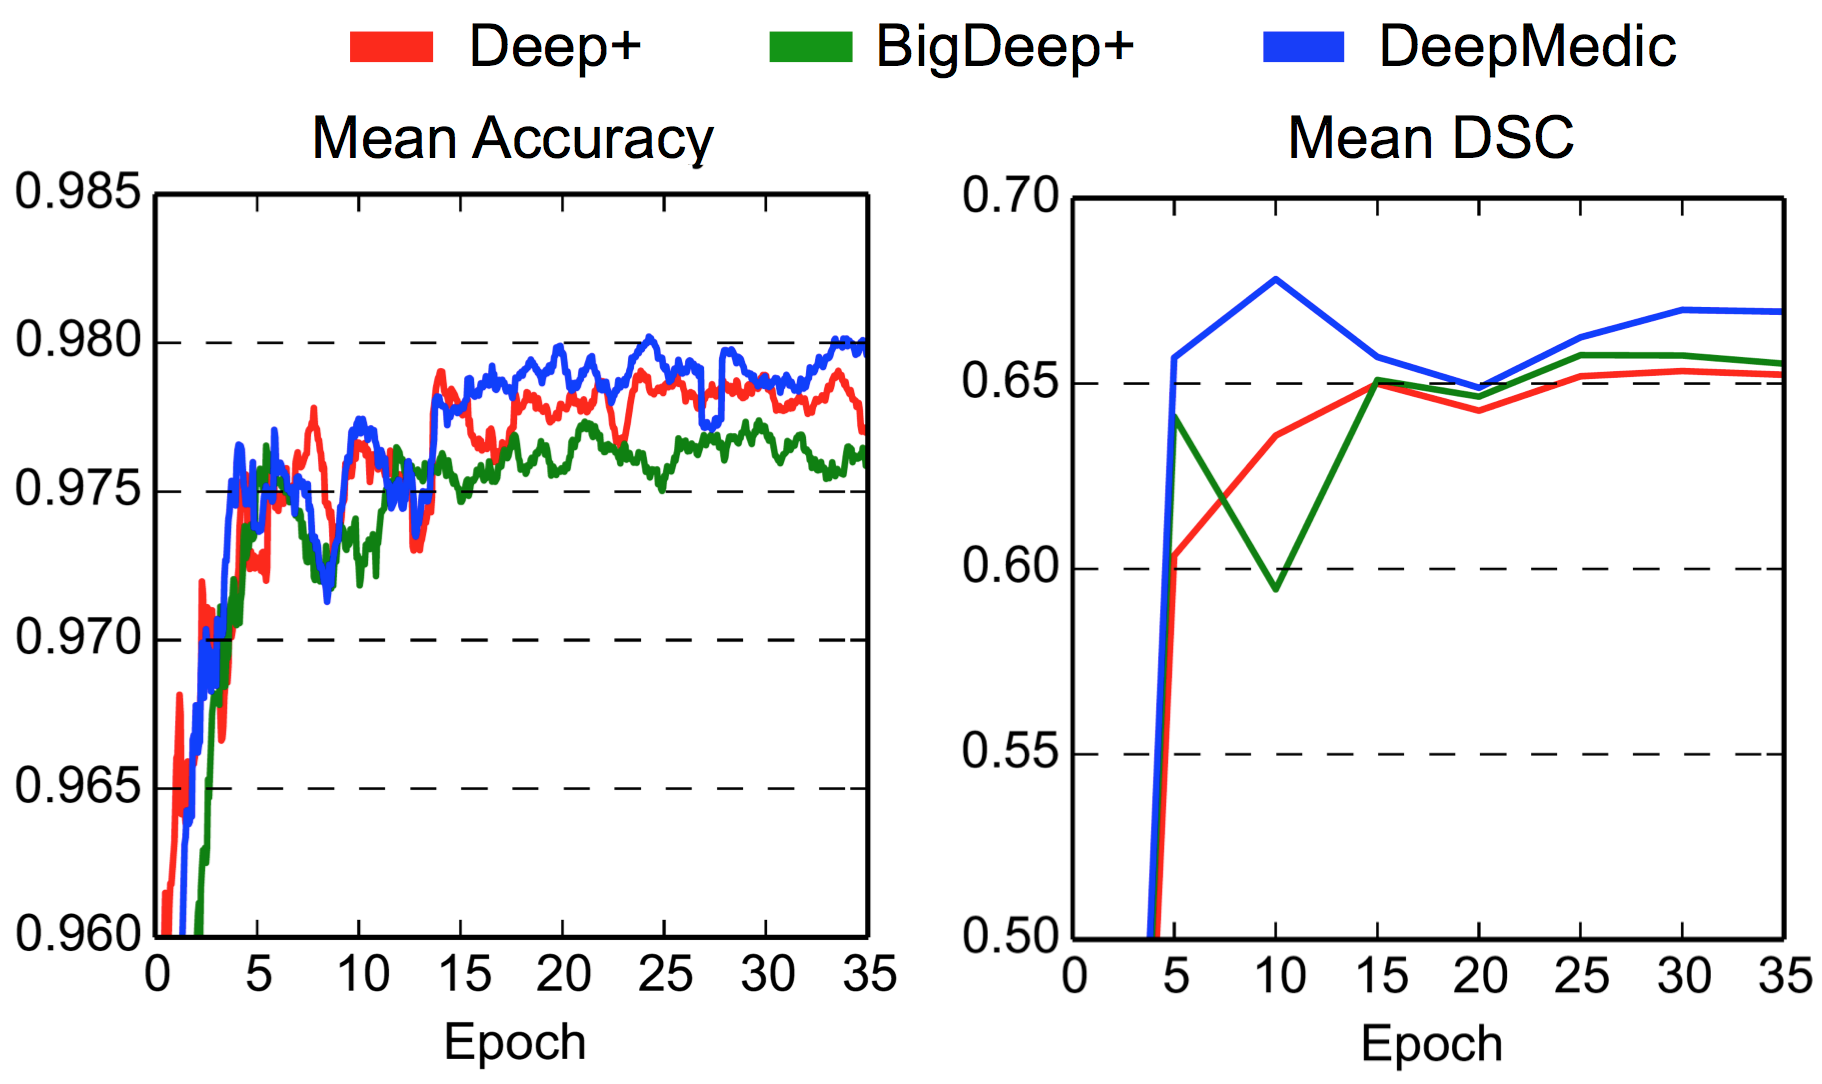
\includegraphics[clip=true, trim=50pt 30pt 140pt 250pt, width=1.0\textwidth]{figures/validationOfArchitecture/multiscale/figureToPut.pdf}
	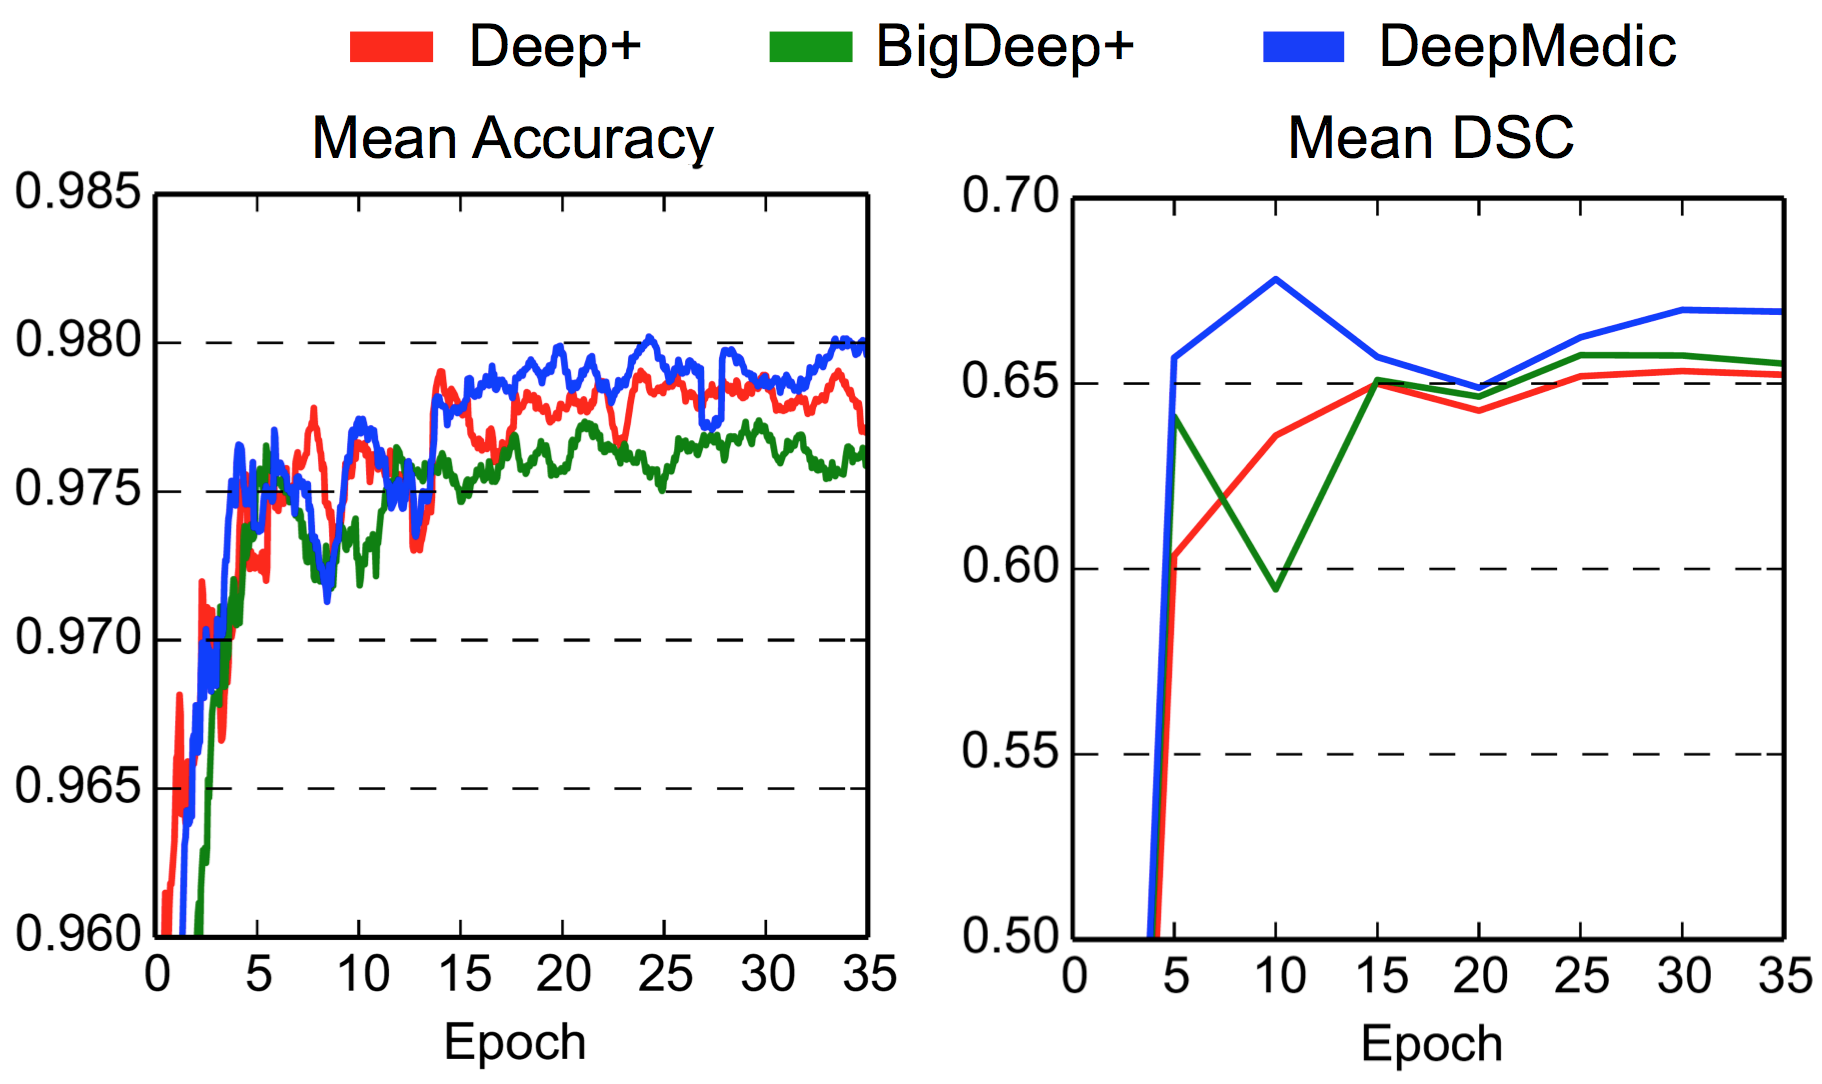
\includegraphics[clip=true, trim=0pt 0pt 0pt 0pt, width=1.0\textwidth]{figures/validationOfArchitecture/multiscale/figureToPut.png}
\end{subfigure}
\caption{Mean accuracy over validation samples and DSC for the segmentation of the validation images, as obtained by a single-scale model (Deep\texttt{+}) and our dual pathway architecture (DeepMedic). We also trained a single-scale model with larger capacity (BigDeep\texttt{+}), similar to the capacity of DeepMedic. DeepMedic yields best performance by capturing greater context, while BigDeep\texttt{+} seems to suffer from over-fitting.
}
\label{fig:multiscaleExperiment}
\end{figure}
%\vspace{-1pt} %takes away some white space before figure